With the term Artificial Intelligence (\textbf{AI}) we refer to the intelligence demonstrated by machines that mimic cognitive functions that humans associate with other human minds, such as learning and problem-solving.
Machine learning (\textbf{ML}) is a subset of AI compound by algorithms and statistical models that computer systems use to perform specific tasks without using explicit instructions, relying on patterns and inference instead.
There are 3 types of ML: supervised learning, self-supervised (or unsupervised learning) and reinforcement learning.
Deep Learning (\textbf{DL}) is a subset of ML that uses artificial neural networks to model and understand complex patterns and relationships in data.
Anyway, everything is based on curve fitting, linear or non-linear, and the goal is to minimize the error between the predicted output and the actual output.
For this reason, studying the causation is important to make sense of data, to understand how to have an effect on a system and to guide actions and policies.
In the Figure \ref{fig:ai_set.png} you can see the relationship between AI, ML and DL.

\begin{figure}[ht]
    \centering
    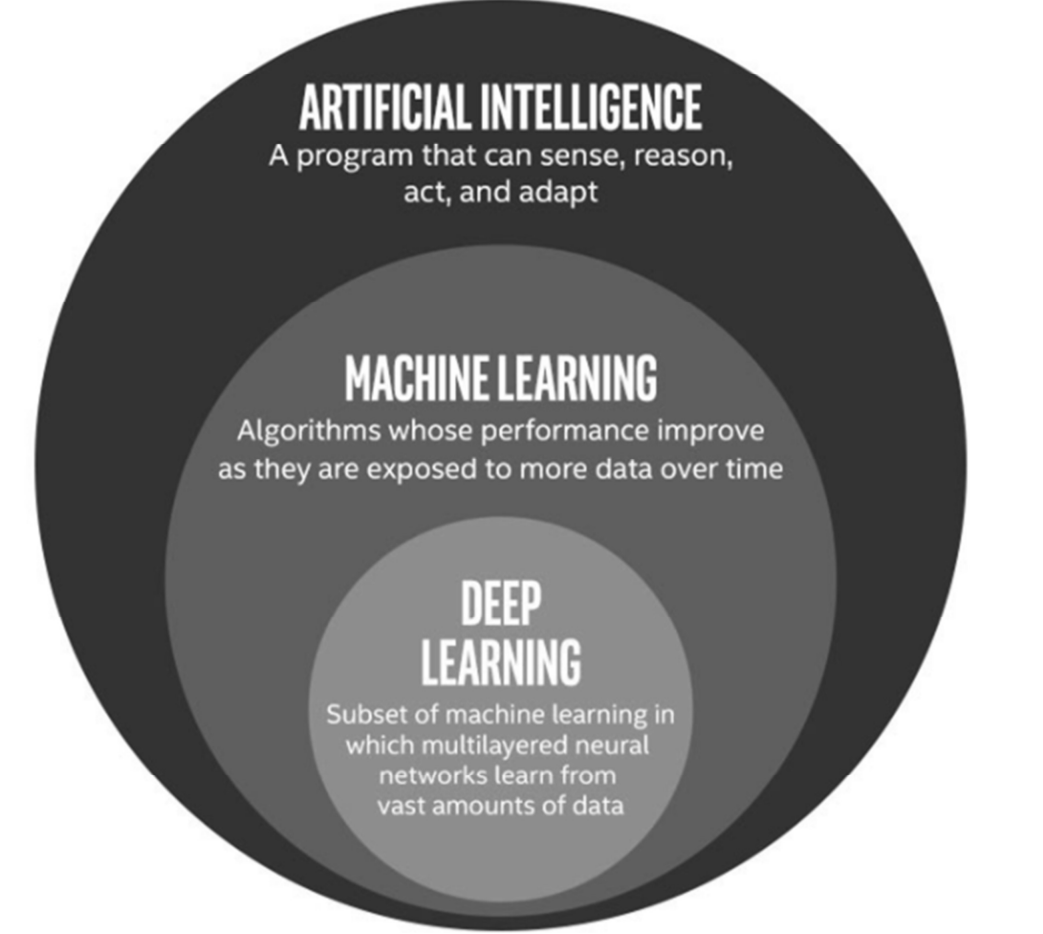
\includegraphics[width=0.6\textwidth]{immagini/ai_set.png}
    \caption{The set of AI, ML and DL.}
    \label{fig:ai_set.png}
\end{figure}

\section{Simpson's Paradox}
\label{simp_para_cap}
Statistical phenomenon in which an observed trend in different groups disappears or reverses when the groups are combined, so this can lead to an evaluation error.
So data alone aren't enough to fully understand a system and  to make decisions (\textbf{correlation is not causation}).
In Fig. \ref{fig:simp_para_exe.png} there is an example, if we consider only the combined data the drug appears to be harmful: only 78\% of the patients recovered 
compared to 83\% of the patients that didn't take the drug, but if we consider the data divided by gender, we can see that the drug is actually beneficial for both men and women.
\begin{figure}[ht]
    \centering
    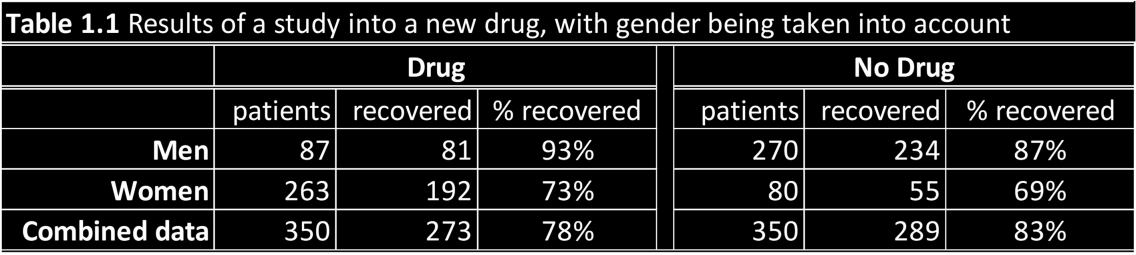
\includegraphics[width=0.6\textwidth]{immagini/simp_para_exe.png}
    \caption{Simpson's Paradox - Example.}
    \label{fig:simp_para_exe.png}
\end{figure}

\subsection{The Pitfall of Blind Data Segregation}

A common mistake is assuming that segregating data by any available variable always yields 
the correct decision. 
\newline
Indeed, as shown in the following example (Fig \ref{fig:simp_para_exe2.png}) is not correct to just segregate the data whenever is possible. 
In this example we were considering the effect of a drug on the recovery of patients with an High BP by lowering the BP, unfortunately the drug has also a toxic effect.
The segregated data shows that without taking the drug the recovery rate is higher for both groups (Low BP and High BP). 
However considering only the subpopulations in this case would introduce a bias as we would only see the drug's toxic effect. In general population, the drug might improve recovery rates because it has an effect on BP, 
a person with High BP has 73\% of recovery rate without taking the drug, but if he takes the drug he could lower his BP and recover with 87\% of probability.
If we consider only the subpopulations  

\begin{figure}[ht]
    \centering
    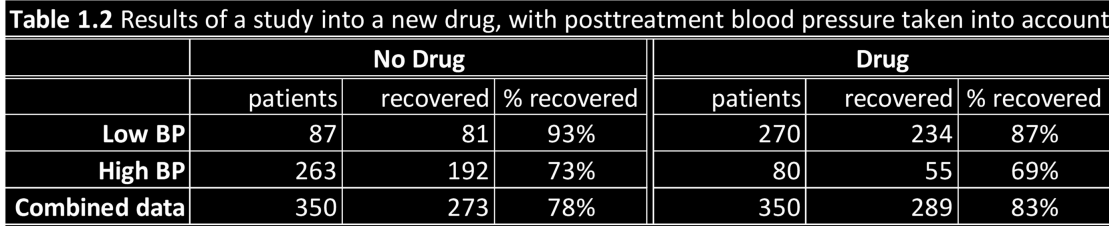
\includegraphics[width=0.6\textwidth]{immagini/simp_para_exe2.png}
    \caption{Simpson's Paradox - Second Example.}
    \label{fig:simp_para_exe2.png}
\end{figure}

\section{Ladder of Causation}
\subsubsection{Level of Association}
Prediction based on passive observations, for instace an marketing director asking if a customer
who bought a toothpase is likely to buy a toothbrush.
\subsubsection{Level of Intervention}
Actionable predictions based on interventions, for instance, a marketing director asking if a customer
is likely to buy a toothbrush if offered a discount.
\subsubsection{Level of Counterfactual}
Predictions based on hypothetical outcomes of events that happened in the past. 
For instance, a marketing director asking if a customer would have bought a toothbrush if he had not bought a toothpaste.